\documentclass[10pt,border=3mm]{standalone}
\usepackage{tikz}

\begin{document}

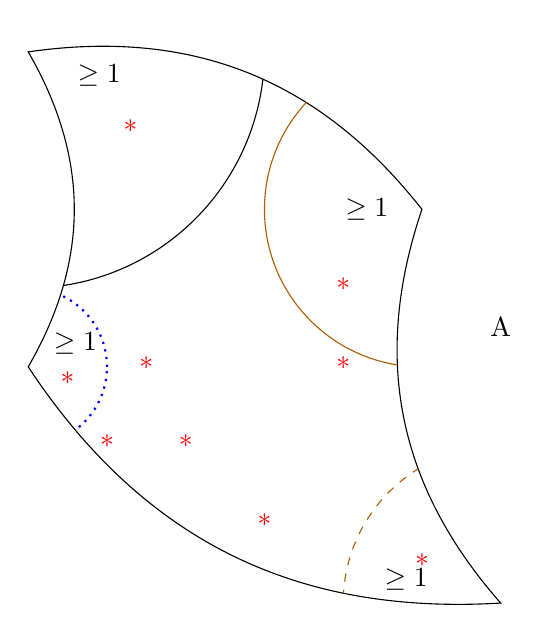
\begin{tikzpicture}
    [ci/.style={draw=black!30!orange}]

    % ~~~ coordinates ~~~~~~~~
    \coordinate (A) at (4,3);
    \coordinate (B) at (5,-2);
    \coordinate (C) at (-1,1);
    \coordinate (D) at (-1,5);

    % ~~~ labels ~~~~~~~~~~~~~
    \node at (5,1.5) {A};
    \node at (A) [xshift=-7mm] {$\ge 1$};
    \node at (B) [xshift=-12mm,yshift=3mm] {$\ge 1$};
    \node at (C) [xshift=+6mm,yshift=3mm] {$\ge 1$};
    \node at (D) [xshift=+9mm,yshift=-3mm] {$\ge 1$};
    
    % ~~~ clipping path ~~~~~~~~~~
    \draw [clip] (A)to [bend right]  (B) 
                    to [bend left]   (C) 
                    to [bend right]  (D)
                    to [bend left]  cycle;
    
    % ~~~ venn-circles ~~~~
    \draw [ci]                  (A) circle[radius=2cm];
    \draw [ci,dashed]           (B) circle[radius=2cm];
    \draw [blue,dotted,thick]   (C) circle[radius=1cm];
    \draw                       (D) circle[radius=3cm];
    
    % ~~~ points ~~~~
    \foreach \x/\y in {0/0, 1/0, .5/1, 3/1, 3/2, 2/-1, 4/-1.5, .3/4, -.5/.8}
        \node [red] at (\x,\y){*};% text for simplicity


\end{tikzpicture}


\end{document}